\documentclass[10pt, a4paper]{article}
    \usepackage[utf8]{inputenc}
    %\usepackage[english, spanish]{babel}
    %\usepackage{fullpage} % changes the margin
    \usepackage{graphicx} 
    \usepackage{enumitem} 
    \usepackage{chngcntr}
    \counterwithin{figure}{section}
    \renewcommand{\thesection}{\arabic{section}} 
    \renewcommand{\thesubsection}{\thesection.\arabic{subsection}}
    \renewcommand{\baselinestretch}{1.5}

    \usepackage{amsmath}
    \usepackage{mathptmx}
    \usepackage[spanish]{babel}
    \usepackage{amssymb}
    \usepackage{makeidx}
    \usepackage{float}
    \pagenumbering{arabic}
    \usepackage[left=25mm, right=25mm, top=25mm, bottom=25mm]{geometry}

\begin{document}

    \begin{titlepage}
        \centering
        {\scshape\Large Universidad Central de Venezuela \par}
        {\scshape\Large Facultad de ingenier\'ia \par}
        {\scshape\Large Escuela de ingenier\'ia El\'ectrica \par}
        {\scshape\Large Departamento de Electr\'onica, Computaci\'on y Control \par}

        \vspace{6cm}
        {\Large\bfseries PRE LAB 3 - Polarización del BJT\par}
        \vspace{5cm}

        \vfill
        \begin{flushright}
            Estudiante:\par
            Ricardo Santana C.I.29571461 \par
            \vspace{1cm}
            Auxiliar docente:\par
            José Tovar  
        \end{flushright}
        \vfill
        {\large \today\par}
    \end{titlepage}

    \section{Introducción}

    Entre las diversas estructuras que pueden conformar los semiconductores cabe destacar la del transistor de unión bipolar, conocido por sus siglas en inglés como BJT (Bipolar Junction Transistor), ésta consta de dos uniones pn construidas de manera especial y conectadas en serie, espalda con espalda.

    El transistor consta de tres terminales, estos se denominan emisor (E), base (B) y colector (C); en base a estos el transistor puede implementarse en un circuito con configuración emisor común, base común o colector común, Se experimentará utilizando la configuración emisor común.
    
    Se presentará en el escrito las nociones básicas del BJT, de tal forma que se permita establecer el punto estático de operación que relaciona a la recta de carga y la curva característica del transistor, la cual nos facilita la implementación y diseño de circuitos electrónicos más complejos con transistores.

    \newpage

    \section{Objetivos}

    \subsection{Objetivo General}
    \begin{itemize}
        \item Análizar las características y el funcionamiento del BJT en la configuración emisor común. 
    \end{itemize}

    \subsection{Objetivos Específicos}
    \begin{itemize}
        \item Familiarizar y estudiar topologías básicas de polarización del BJT en la configuración Emisor Común.
        \item Obtener nociones acerca de la polarización del BJT.
        \item Estudiar el punto estático de operación variando el valor de las resistencias del circuito.
        \item Estudiar la recta de carga estática y su relación con las curvas características del transistor.
    \end{itemize}

    \newpage

    \section{Marco Teórico}

    \subsection{Construcción del transistor}

    El transistor es un dispositivo de tres zonas o capas. Podemos tener una zona de material tipo n en medio de dos zonas de material tipo p, en este caso se denomina transistor pnp, o bien tener una zona tipo p con dos zonas tipo n a cada lado, en cuyo caso estaríamos hablando de un transistor npn.

    \begin{figure}[h!]
        \centering
        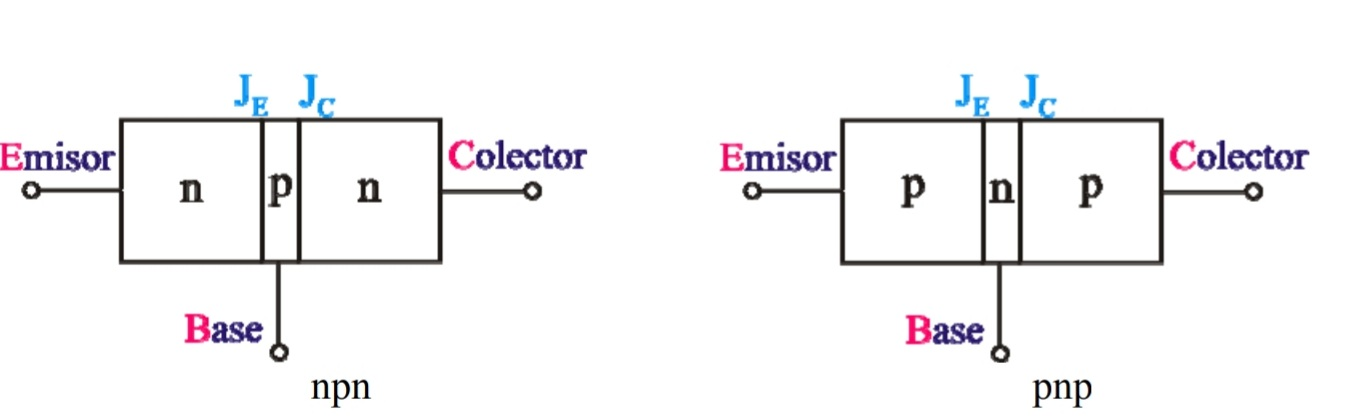
\includegraphics[height=4cm\textwidth]{construcion.jpg}
        \caption{\label{fig:1} Estructura del transistor }
    \end{figure}

    La zona central se denomina base, y las laterales emisor y colector. Cada una de las zonas consta de un terminal por donde extraer las corrientes. Estos terminales se representan por la inicial del nombre de la zona respectiva: E (emitter), B (base) y C (colector).

    \subsection{Simbolos y convenio de signos}

    \begin{figure}[h!]
        \centering
        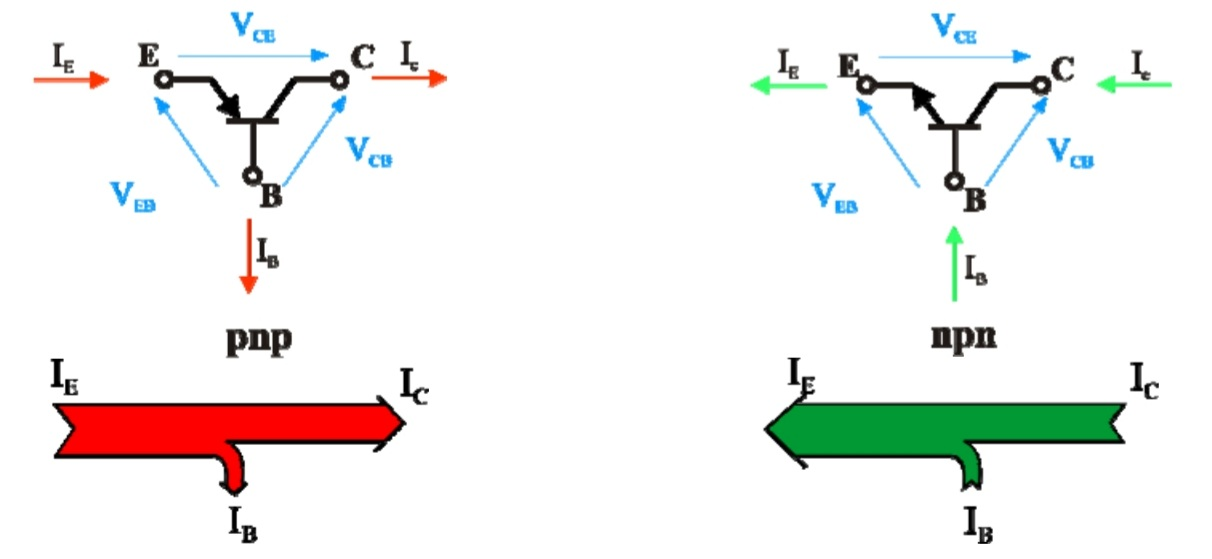
\includegraphics[height=4cm\textwidth]{simbolos.jpg}
        \caption{\label{fig:2} Estructura del transistor }
    \end{figure}

    En la figura aparecen los símbolos que se utilizan para la representación del transistor de unión bipolar. Para las corrientes se han representado los sentidos reales de circulación de las mismas.

    \subsection{zonas de funcionamiento}

    Cuando anteriormente hablábamos de la unión pn veíamos que teníamos dos posibilidades de polarización de la misma, de tal forma que el diodo tenía dos posibles estados o zonas de trabajo: en directa y en inversa. Ahora estamos ante un dispositivo que tiene dos uniones, una unión entre las zonas de emisor y base (que denominaremos a partir de ahora unión de emisor JE) y otra unión entre las zonas de base y colector (de que denominaremos unión de colector JC), cada una de las cuales puede ser polarizada en las dos formas mencionadas anteriormente. Así, desde el punto de vista global del dispositivo tenemos cuatro zonas de funcionamiento posibles en función del estado de polarización de las dos uniones.

    De esta forma, si polarizamos las dos uniones en directa, diremos que el transistor está trabajando en la zona de saturación. En el caso de que la unión de emisor la polaricemos en directa y la unión de colector en inversa, estaremos en la zona activa. Cuando las dos uniones se polarizan en inversa, se dice que el transistor está en la zona de corte. Por último, si la unión de emisor se polariza en inversa y la unión de colector en directa, el transistor se encuentra en activa inversa. De las cuatro zonas, las 3mencionadas en primer lugar son las más interesantes desde el punto de vista del funcionamiento del transistor, siendo la zona activa inversa una zona puramente teórica y sin interés práctico.

    \subsection{Curvas Características en Emisor Común}

    \subsubsection{Curvas características de entrada}

    En la siguiente figura aparecen representados los convenios de tensiones y corrientespositivas que se han tenido en cuenta para representar las distintas curvas.

    \begin{figure}[h!]
        \centering
        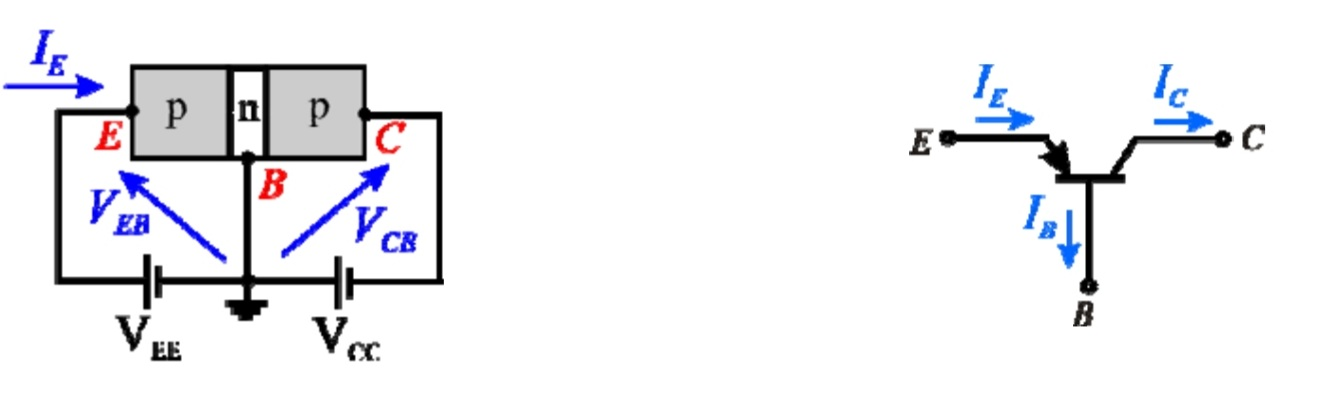
\includegraphics[height=4cm\textwidth]{entrada.jpg}
        \caption{\label{fig:3} Sentido positivo de las variable en la curva característica de entrada del BJT}
    \end{figure}

    Como se puede ver en la figura, no hay una única curva que relacione $I_B$ con $V_{BE}$, sino que hay una familia de curvas en función de $V_{CE}$.

    \begin{figure}[h!]
        \centering
        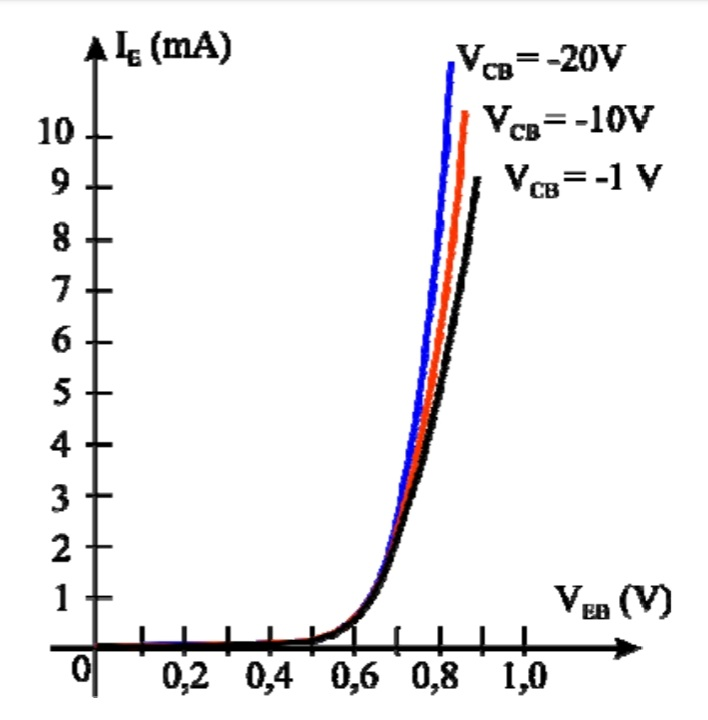
\includegraphics[height=5cm\textwidth]{graficae.jpg}
        \caption{\label{fig:4} Curvas Características de Entrada en Emsior Común para un BJT npn}
    \end{figure}

    \subsubsection{Curvas características de salida}

    \begin{figure}[h!]
        \centering
        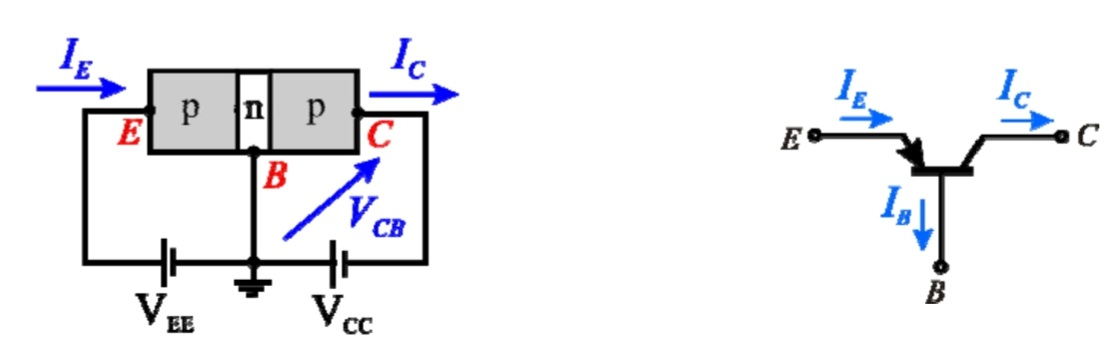
\includegraphics[height=4cm\textwidth]{salida.jpg}
        \caption{\label{fig:5} Sentido positivo de las variable en la curva característica de salida del BJT}
    \end{figure}

    En las características de salida en emisor común se representa
    
    $$I_C = f(V_{CE}, I_C)$$

    Los sentidos positivos de tensiones y corrientes son los que aparecen representados en la figura anterior

    \begin{figure}[h!]
        \centering
        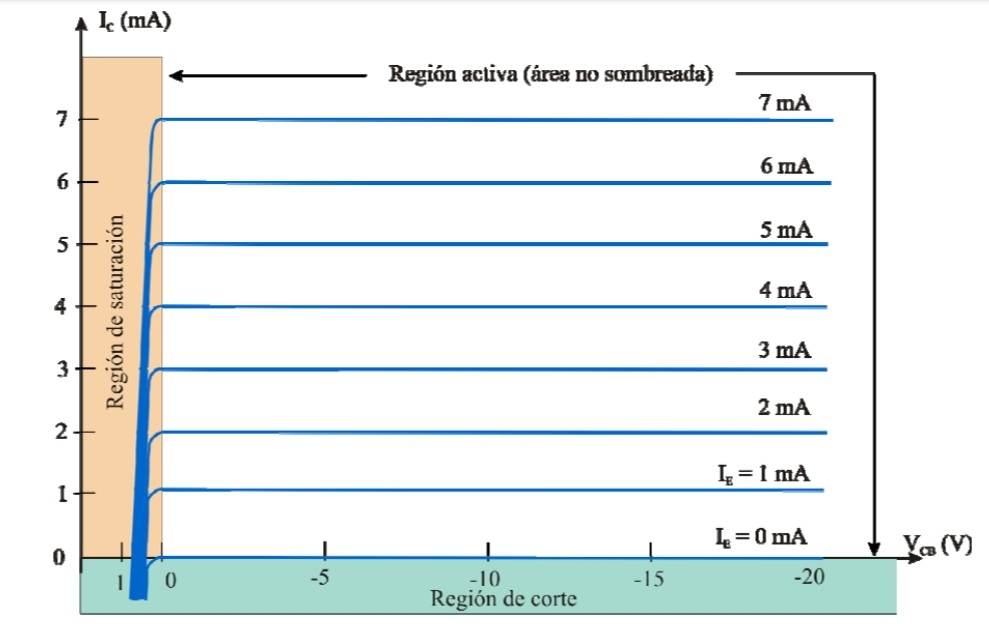
\includegraphics[height=5cm\textwidth]{graficas.jpg}
        \caption{\label{fig:6} Curvas características de salida en Emisor Común en un BJT npn}
    \end{figure}

    \newpage
    \newpage

    \section{Metodología}

    \subsection{Trabajo Previo al Laboratorio}

    \begin{enumerate}
        \item 	Determine el punto estático de operación y obtenga la tensión en cada uno de los terminales (tensión en el Colector ($V_C$), tensión en la Base (VB) y la tensión en el Emisor ($V_E$)) del BJT, para los circuitos de la Figura 7, 8, 9, 10 y 11. El valor de $V_{BE}$ y $\beta$, deben obtenerlo del manual del fabricante según el transistor a utilizar.
    \end{enumerate}

    \subsection{Trabajo de Laboratorio}

    \begin{enumerate}
        \item Mida la tensión en cada uno de los terminales del transistor y obtenga el punto estático de operación para el circuito de la Figura 7, 8 y 9.
        \item Para el circuito de la Figura 10 realice lo siguiente:
        \begin{enumerate}
            \item mida la tensión en cada uno de los terminales del transistor y obtenga el punto estático de operación.
            \item mida la tensión en cada uno de los terminales del transistor y obtenga el punto estático de operación con los siguientes valores de resistencia en el circuito:
            \begin{enumerate}
                \item $RB=82k\Omega, RC=2k\Omega y RE=200\Omega.$
                \item $RB=36k\Omega, RC=2k\Omega y RE=200\Omega.$
                \item $RB=56k\Omega, RC=3k\Omega y RE=200\Omega.$
                \item $RB=56k\Omega, RC=1,3k\Omega y RE=200\Omega.$ 
                \item $RB=56k\Omega, RC=2k\Omega y RE=300\Omega.$
                \item $RB=56k\Omega, RC=2k\Omega y RE=130\Omega.$
            \end{enumerate}
        \end{enumerate}
        \item Para el circuito de la Figura 11 realice lo siguiente:
        \begin{enumerate}
            \item mida la tensión en cada uno de los terminales del transistor y obtenga el punto estático de operación.
            \item mida la tensión en cada uno de los terminales del transistor y obtenga el punto estático de operación con los siguientes valores de resistencia en el circuito:
            \begin{enumerate}
                \item $R1=82k\Omega, R2=10k\Omega, RC=510\Omega y RE=200\Omega.$
                \item $R1=39k\Omega, R2=10k\Omega, RC=510\Omega y RE=200\Omega.$
                \item $R1=56k\Omega, R2=15k\Omega, RC=510\Omega y RE=200\Omega.$
                \item $R1=56k\Omega, R2=6,8k\Omega, RC=510\Omega y RE=200\Omega.$
                \item $R1=56k\Omega, R2=56k\Omega, RC=750\Omega y RE=200\Omega.$
                \item $R1=56k\Omega, R2=56k\Omega, RC=360\Omega y RE=200\Omega.$
            \end{enumerate}
        \end{enumerate}
        \item 	Para el circuito de la Figura 12, varíe el potenciómetro de un extremo a otro, observe que ocurre con la tensión en cada uno de los terminales del transistor y el punto estático de operación. Anote en cada extremo la tensión en cada uno de los terminales del transistor y obtenga el punto estático de operación. Coloque el potenciómetro aproximadamente en la mitad de su recorrido y realice las mediciones respectivas.
    \end{enumerate}

    \newpage

    \begin{figure}[h!]
        \centering
        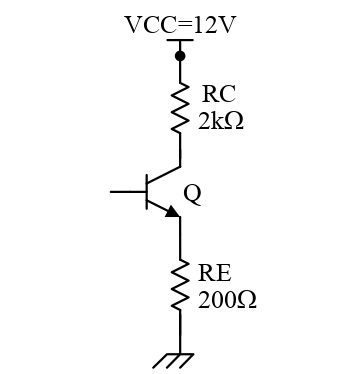
\includegraphics[height=5cm\textwidth]{circuito1.jpg}
        \caption{\label{fig:7} Circuito 1}
    \end{figure}

    \begin{figure}[h!]
        \centering
        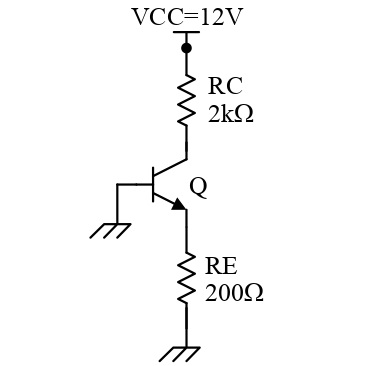
\includegraphics[height=5cm\textwidth]{circuito2.jpg}
        \caption{\label{fig:8} Circuito 2}
    \end{figure}

    \begin{figure}[h!]
        \centering
        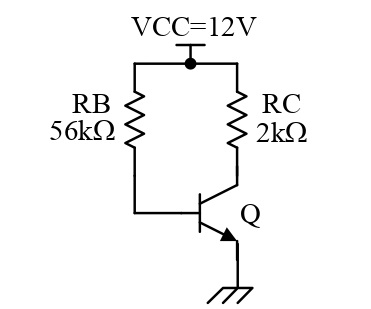
\includegraphics[height=5cm\textwidth]{circuito3.jpg}
        \caption{\label{fig:9} Circuito 3}
    \end{figure}

    \newpage

    \begin{figure}[h!]
        \centering
        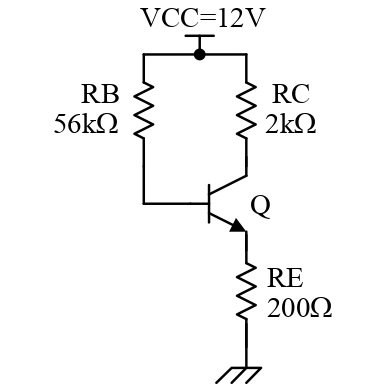
\includegraphics[height=5cm\textwidth]{circuito4.jpg}
        \caption{\label{fig:10} Circuito 4}
    \end{figure}

    \begin{figure}[h!]
        \centering
        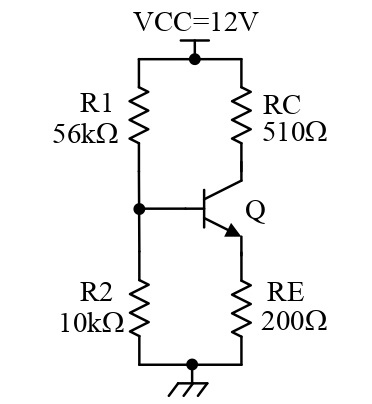
\includegraphics[height=5cm\textwidth]{circuito5.jpg}
        \caption{\label{fig:11} Circuito 5}
    \end{figure}

    \begin{figure}[h!]
        \centering
        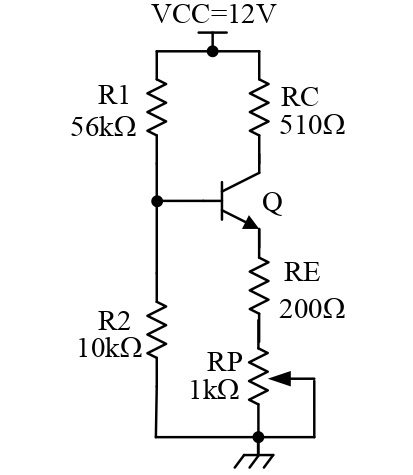
\includegraphics[height=5cm\textwidth]{circuito6.jpg}
        \caption{\label{fig:12} Circuito 6}
    \end{figure}

    \newpage

    \section{Cálculos prévios}

    Se trabajará con el transistor npn PN2222A, el cual posee las siguientes especificaciones:

    
    \begin{figure}[h!]
        \centering
        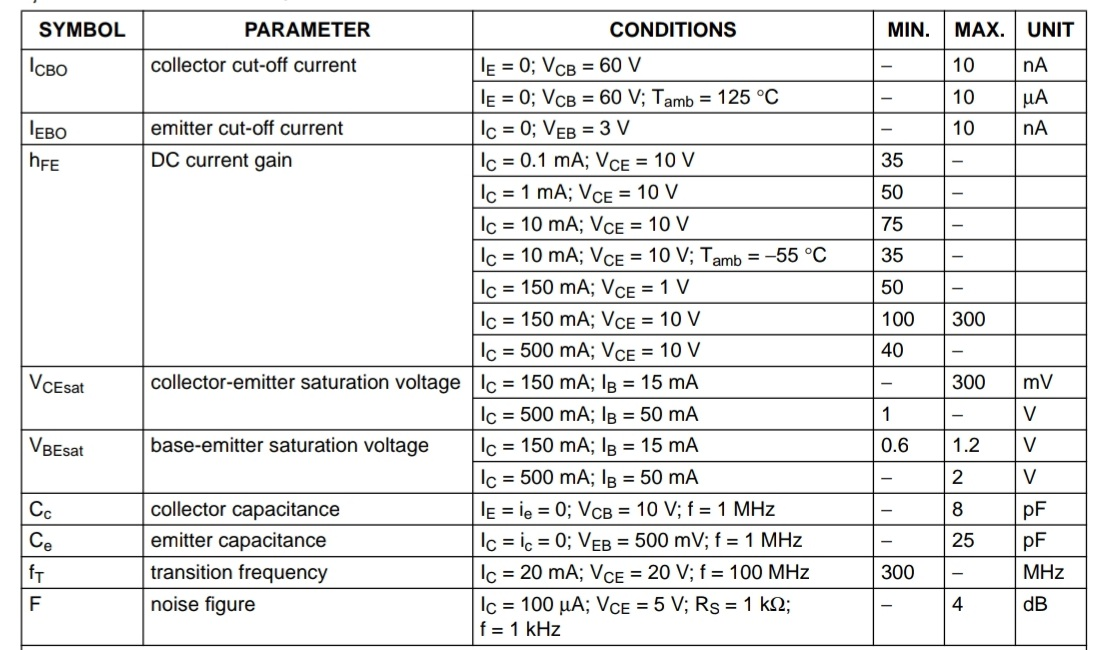
\includegraphics[height=7cm\textwidth]{especificaciones.jpg}
    \end{figure}
    

    de las cuales se deduce que:
    $$\beta = h_{FE} = 100 \; @ \; I_C = 150mA; \; V_{CE} = 10V \; (mínimo)$$
    $$V_{BEsat} = 0.6V \; @ \; I_C = 150mA; \; I_B = 15mA \; (mínimo)$$

    \subsection{Analisis del circuito de la figura 7}

    \begin{figure}[h!]
        \centering
        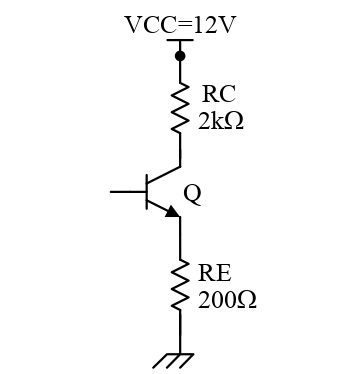
\includegraphics[height=5cm\textwidth]{circuito1.jpg} \par
        Circuito 1
        %\caption{\label{fig:7} Circuito 1}
    \end{figure}

    $V_B$ : indeterminado (circuito abierto) $\rightarrow$ asumiendo $V_B = 0V$
    Como $I_C = \beta I_B \longrightarrow I_C = 0A$, por lo tanto
    $$V_C = 12V$$
    Además $I_E = (\beta + 1)I_B \longrightarrow I_E = 0A$, por lo tanto
    $$V_E = 0V$$

    $$V_{CE} = V_C - V_E = 12V$$

    El transistor no se encuentra en la zona de saturación, entonces el punto de operación de la figura 7 es:

    $$Q : (12V, 0A)$$

    \subsection{Analisis del circuito de la figura 8}

    \begin{figure}[h!]
        \centering
        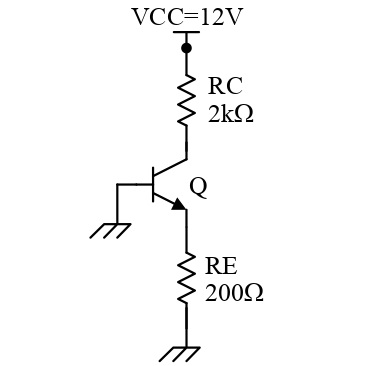
\includegraphics[height=5cm\textwidth]{circuito2.jpg}
        %\caption{\label{fig:5} Circuito 5}
    \end{figure}

    estimando $V_C > 0 \rightarrow V_B = 0 < V_C$, por tanto el transistor está polarizado inversamente, que indica que se encuentra en su zona de corte, entonces

    $$V_B = 0V$$

    Como $I_C = \beta I_B \longrightarrow I_C = 0A$, por lo tanto
    $$V_C = 12V$$
    Además $I_E = (\beta + 1)I_B \longrightarrow I_E = 0A$, por lo tanto
    $$V_E = 0V$$

    $$V_{CE} = V_C - V_E = 12V$$

    El transistor no se encuentra en la zona de saturación, entonces el punto de operación de la figura 7 es:

    $$Q : (12V, 0A)$$

    \subsection{Analisis del circuito de la figura 9}

    \begin{figure}[h!]
        \centering
        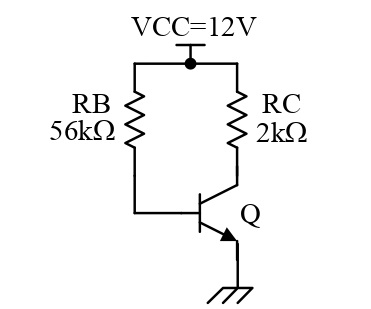
\includegraphics[height=5cm\textwidth]{circuito3.jpg}
        %\caption{\label{fig:5} Circuito 5}
    \end{figure}

    aplicando ley de tensiones de Kirchoff se tiene

    $$R_BI_B + V_{BE} = V_{CC}$$

    despejando $I_B$

    $$I_B = \frac{V_{CC} - V_{BE}}{R_B}$$

    sustituyendo valores

    $$I_B = \frac{12V - 0.6V}{56k\Omega} = 0.204mA$$

    aplicando ley de tensiones de Kirchoff a la malla faltante

    $$R_CI_C + V_{CE} = V_{CC}$$

    sabiendo que $I_C = \beta I_B$

    $$R_C\beta I_B + V_{CE} = V_{CC}$$

    despejando $V_{CE}$

    \begin{equation}
        V_{CE} = V_{CC} - R_C\beta I_B
    \end{equation}

    sustituyendo valores

    $$V_{CE} = 12V - 2k\Omega (100) (0.204mA) = -38.8V$$

    El transistor no se encuentra en estado de saturacion, entonces aplicando la lógica de los circuitos 1 y 2:

    \begin{array}{rcl}
        V_C & = & 12V \\
        V_B & = & 12V \\
        V_E & = & 0V \\
        V_{CE} & = & 12V \\
        Q & : & (12V, 0A)
    \end{array}

    por convención de signos los valores que puede llegar a tomar $V_{CE}$ quedan establecidos  en $V_{CE} > 0$

    por tanto si $V_{CE} = 0$ en (1):

    $$0 = 12V - R_C (100) (0.204mA)$$
    $$R_C = 588\Omega$$

    Entonces se debría cumplir que para $R_C < 588\Omega$ el transistor se encuentra saturado y circula corriente por el circuito

    \subsection{Analisis del circuito de la figura 10}

    \begin{figure}[h!]
        \centering
        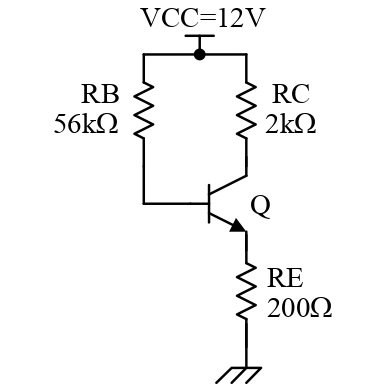
\includegraphics[height=5cm\textwidth]{circuito4.jpg}
        %\caption{\label{fig:5} Circuito 5}
    \end{figure}

    aplicando ley de tensiones de Kirchoff se tiene

    $$R_BI_B + V_{BE} + R_EI_E= V_{CC}$$

    sabiendo que $I_E = (\beta+1)I_B$

    $$R_BI_B + V_{BE} + R_E(\beta+1)I_B= V_{CC}$$

    despejando $I_B$

    $$I_B = \frac{V_{CC} - V_{BE}}{R_B + R_E(\beta + 1)}$$

    sustituyendo valores

    $$I_B = \frac{12V - 0.6V}{56k\Omega + 200\Omega (100 + 1)} = 0.150mA$$

    aplicando ley de tensiones de Kirchoff a la malla faltante

    $$R_CI_C + V_{CE} + R_EI_E = V_{CC}$$

    sabiendo que $I_C = \beta I_B$ y $I_E = (\beta + 1)I_B$

    $$R_C\beta I_B + V_{CE} + R_E(\beta + 1)I_B= V_{CC}$$

    despejando $V_{CE}$

    \setcounter{equation}{1}
    \begin{equation}
        V_{CE} = V_{CC} - R_C\beta I_B - R_E(\beta + 1)I_B
    \end{equation}

    sustituyendo valores

    $$V_{CE} = 12V - 2k\Omega (100) (0.204mA) - 200 \Omega (100 + 1)(0.150mA) = -31.8V$$

    El transistor no se encuentra en estado de saturacion, entonces aplicando la lógica de los circuitos 1 y 2:

    \begin{array}{rcl}
        V_C & = & 12V \\
        V_B & = & 12V \\
        V_E & = & 0V \\
        V_{CE} & = & 12V \\
        Q & : & (12V, 0A)
    \end{array}

    por convención de signos los valores que puede llegar a tomar $V_{CE}$ quedan establecidos  en $V_{CE} > 0$

    por tanto si $V_{CE} = 0$ en (2):

    $$0 = 12V - R_C (100) (0.204mA) - R_E (100 + 1)(0.150mA)$$
    $$0.0204R_C + 0.0151R_E < 12$$

    Quedando así un sistema compatible indeterminado de una ecuación con dos incognitas, en el cual se pueden variar los valores de las resistencias de manera que el transistor se sature.

    \subsection{Analisis del circuito de la figura 11}

    \begin{figure}[h!]
        \centering
        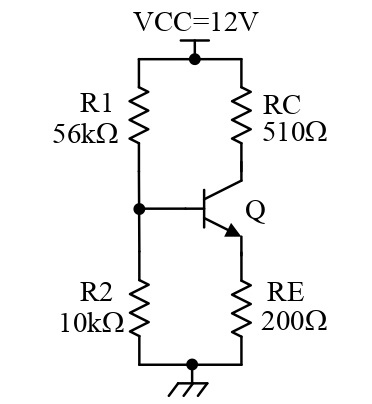
\includegraphics[height=5cm\textwidth]{circuito5.jpg}
        %\caption{\label{fig:5} Circuito 5}
    \end{figure}

    Calculando equivalente de thevelin entre la base del transistor y la referencia

    $$R_{Th} = R_1 // R_2 = 56k\Omega // 10k\Omega = 8.48k\Omega$$
    
    por divisor de voltaje

    $$V_{Th} = \frac{R_2}{R_1 + R_2} V_{CC} = \frac{10k\Omega}{56k\Omega + 10k\Omega} (12V) = 1.81V$$

    \begin{figure}[h!]
        \centering
        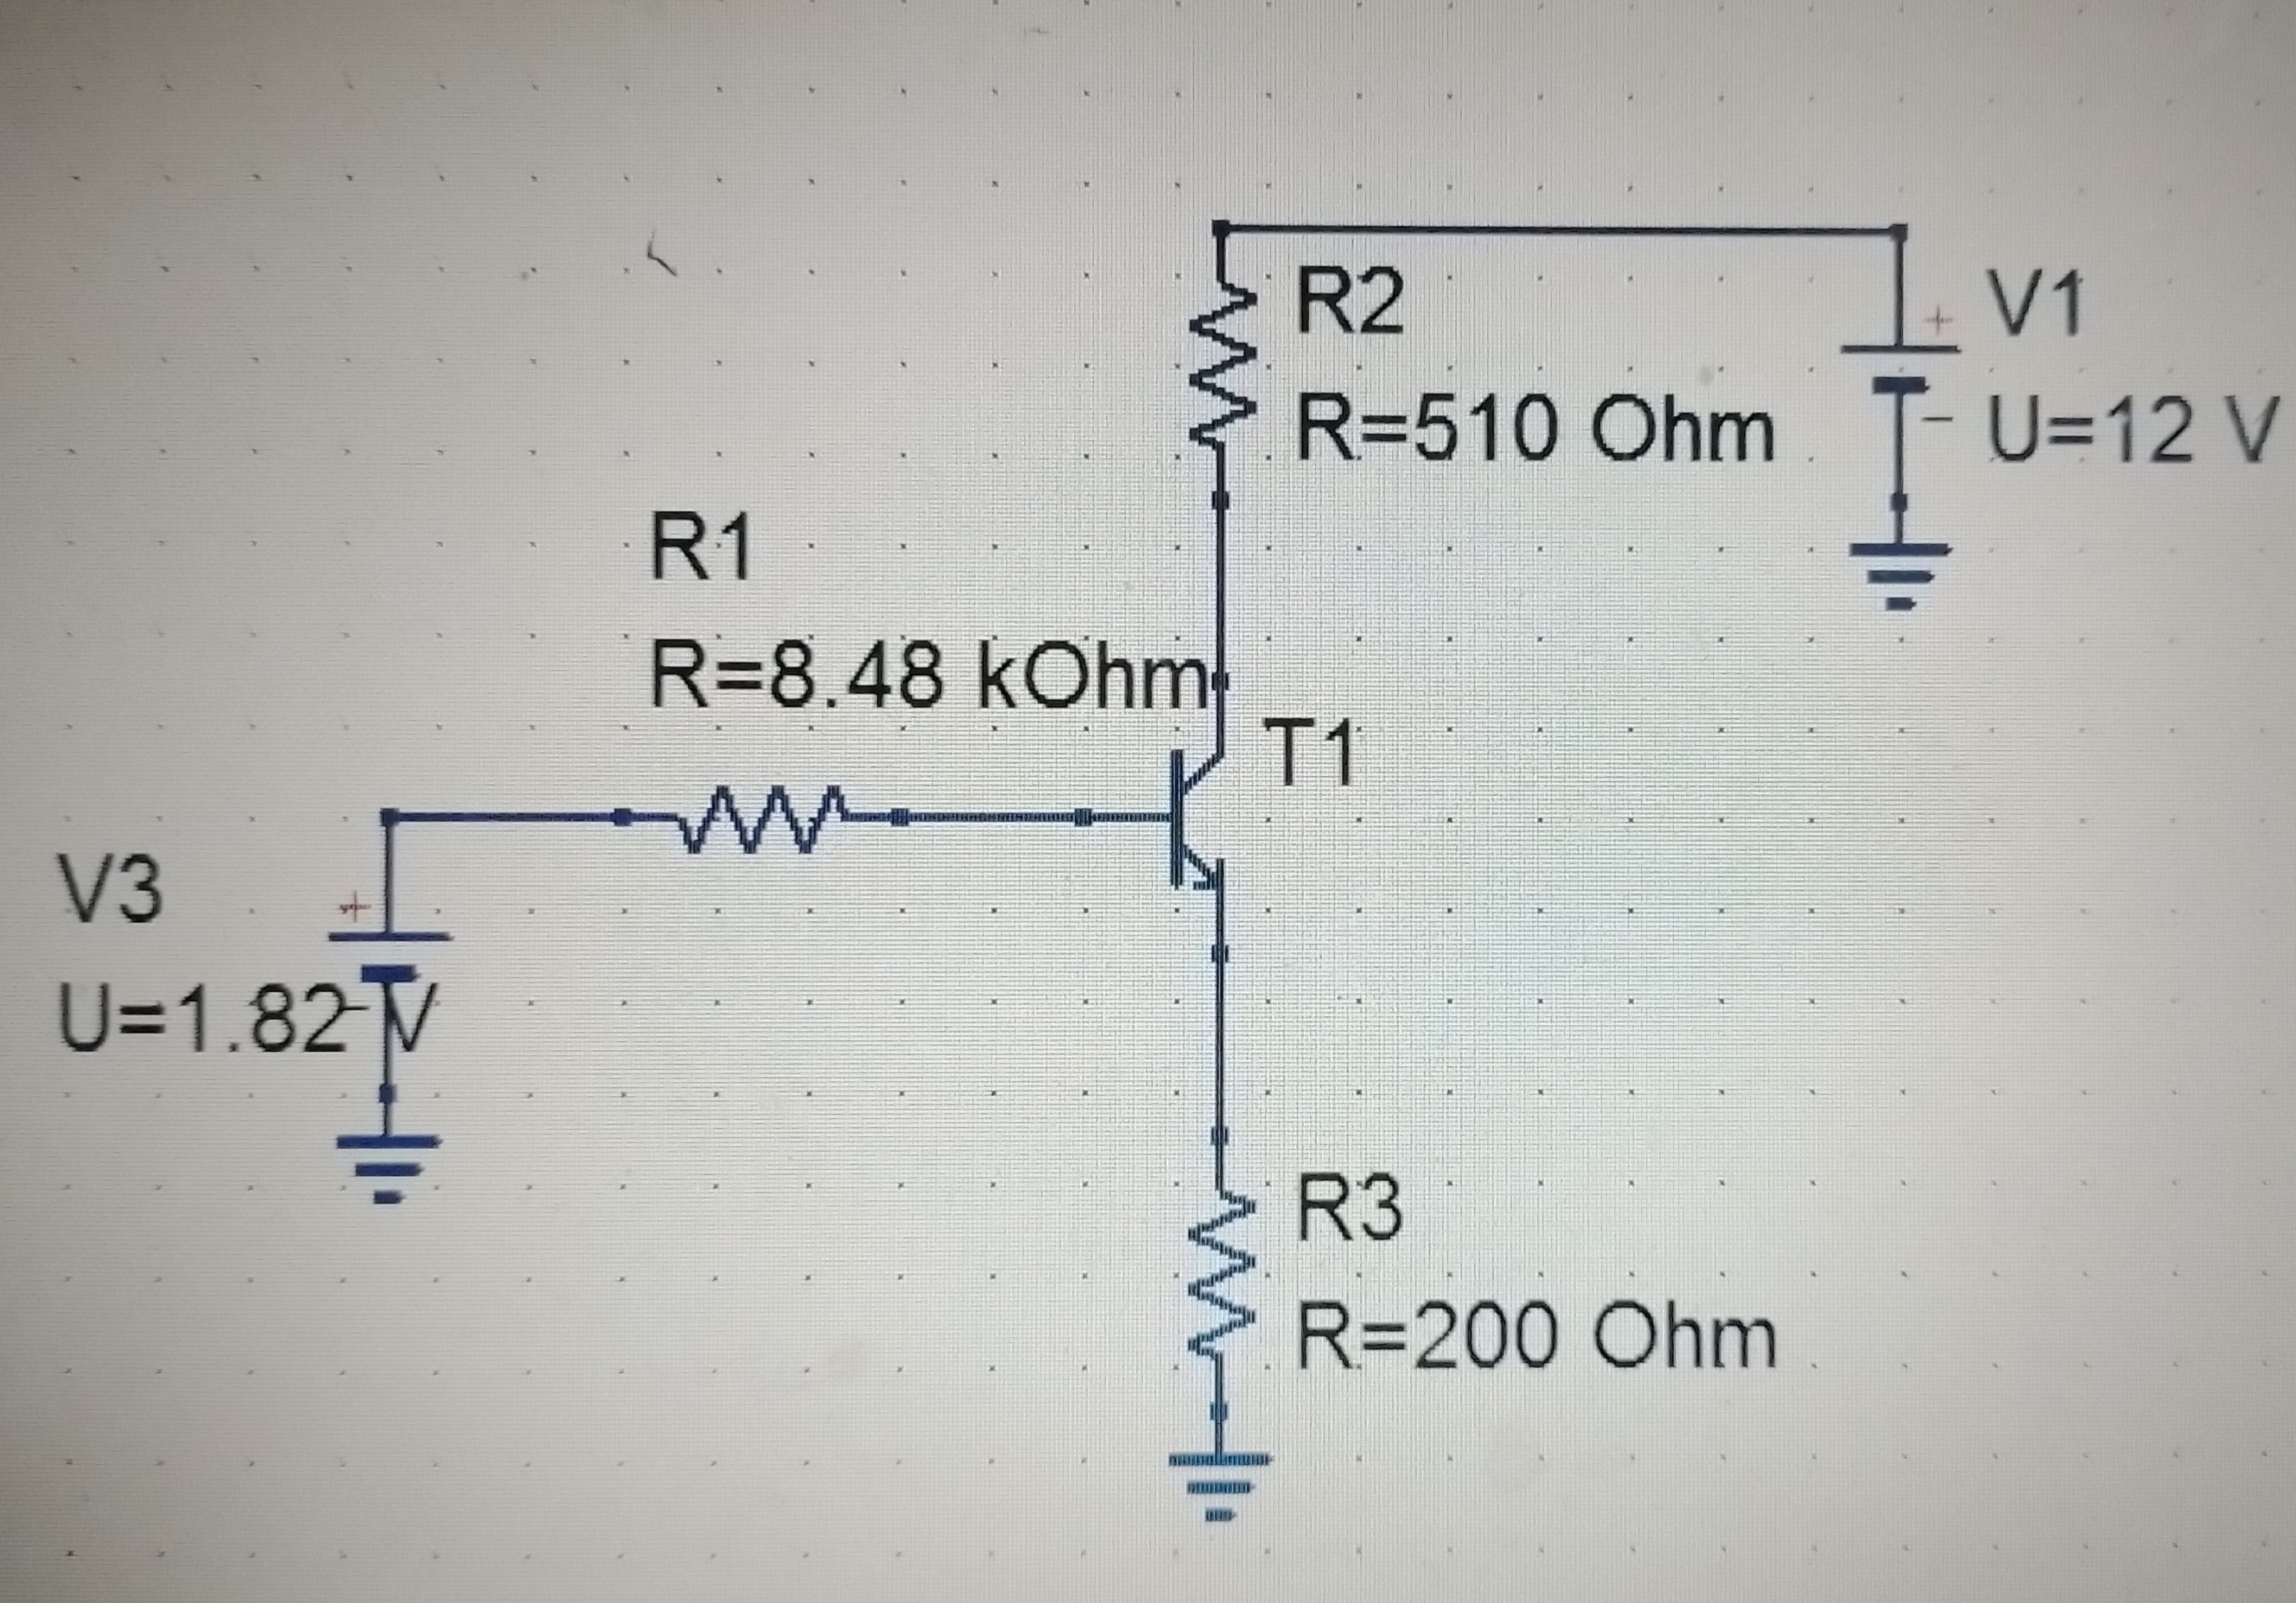
\includegraphics[height=5cm\textwidth]{thevelin5.jpg} \par
        \caption{\label{fig:13} Circuito 5 con equivalente de Thevelin}
    \end{figure}

    aplicando ley de tensiones de Kirchoff

    $$R_{Th}I_B + V_{BE} + R_EI_E = V_{Th}$$

    si $I_E = (\beta + 1)I_B$, entonces

    $$R_{Th}I_B + V_{BE} + R_E(\beta + 1)I_B = V_{Th}$$

    $$I_B = {V_{Th} - V{BE} \over R_{Th} + R_E(\beta + 1)}$$

    Sustituyendo valores

    $$I_B = {1.82V - 0.6V \over 8,48k\Omega + 200\Omega(100 + 1)} = 0.043mA$$

    sabiendo que $I_C = \beta I_B$

    $$I_C = 100(0.043mA) = 4.3mA$$

    por otra parte

    $$I_E = (\beta + 1)I_B = (100 + 1)0.043mA = 4.343mA$$

    aplicando ley de tensiones de Kirchoff a la otra malla

    $$R_{C}I_C + V_{CE} + R_EI_E = V_{CC}$$

    $$V_{CE} = V_{CC} - R_{C}I_C - R_EI_E$$

    sustituyendo

    $$V_{CE} = 12V - 510\Omega (4.3mA) - 200\Omega (4.343mA) = 8.94V$$

    por ley de ohm

    $$V_E = R_EI_E = 200\Omega (4.343mA) = 0.87V$$

    además

    $$V_B = V_{BE} + V_E = 0.6V + 0.87V = 1.47V$$

    $$V_C = V_{CE} + V_E = 8.94V + 0.87V = 9.81V$$

    punto de operacion

    $$Q = (8.94V, 4.30mA)$$

    \subsection{Analisis del circuito de la figura 12}

    \begin{figure}[h!]
        \centering
        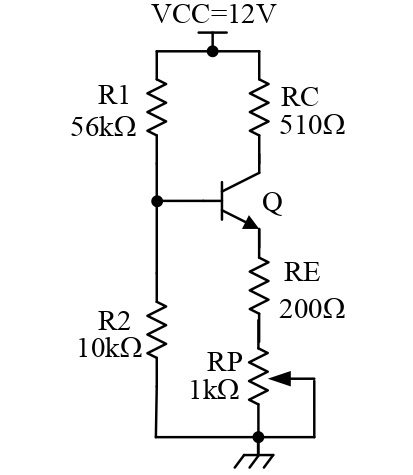
\includegraphics[height=5cm\textwidth]{circuito6.jpg}
        %\caption{\label{fig:5} Circuito 5}
    \end{figure}

    Se aplicará una lógica semejante al circuito anterior, donde:

    $$R_{Ecircuito5} = R_{Ecircuito6} + R_P$$

    Calculando equivalente de thevelin entre la base del transistor y la referencia

    $$R_{Th} = R_1 // R_2 = 56k\Omega // 10k\Omega = 8.48k\Omega$$
    
    por divisor de voltaje

    $$V_{Th} = \frac{R_2}{R_1 + R_2} V_{CC} = \frac{10k\Omega}{56k\Omega + 10k\Omega} (12V) = 1.81V$$

    \begin{figure}[h!]
        \centering
        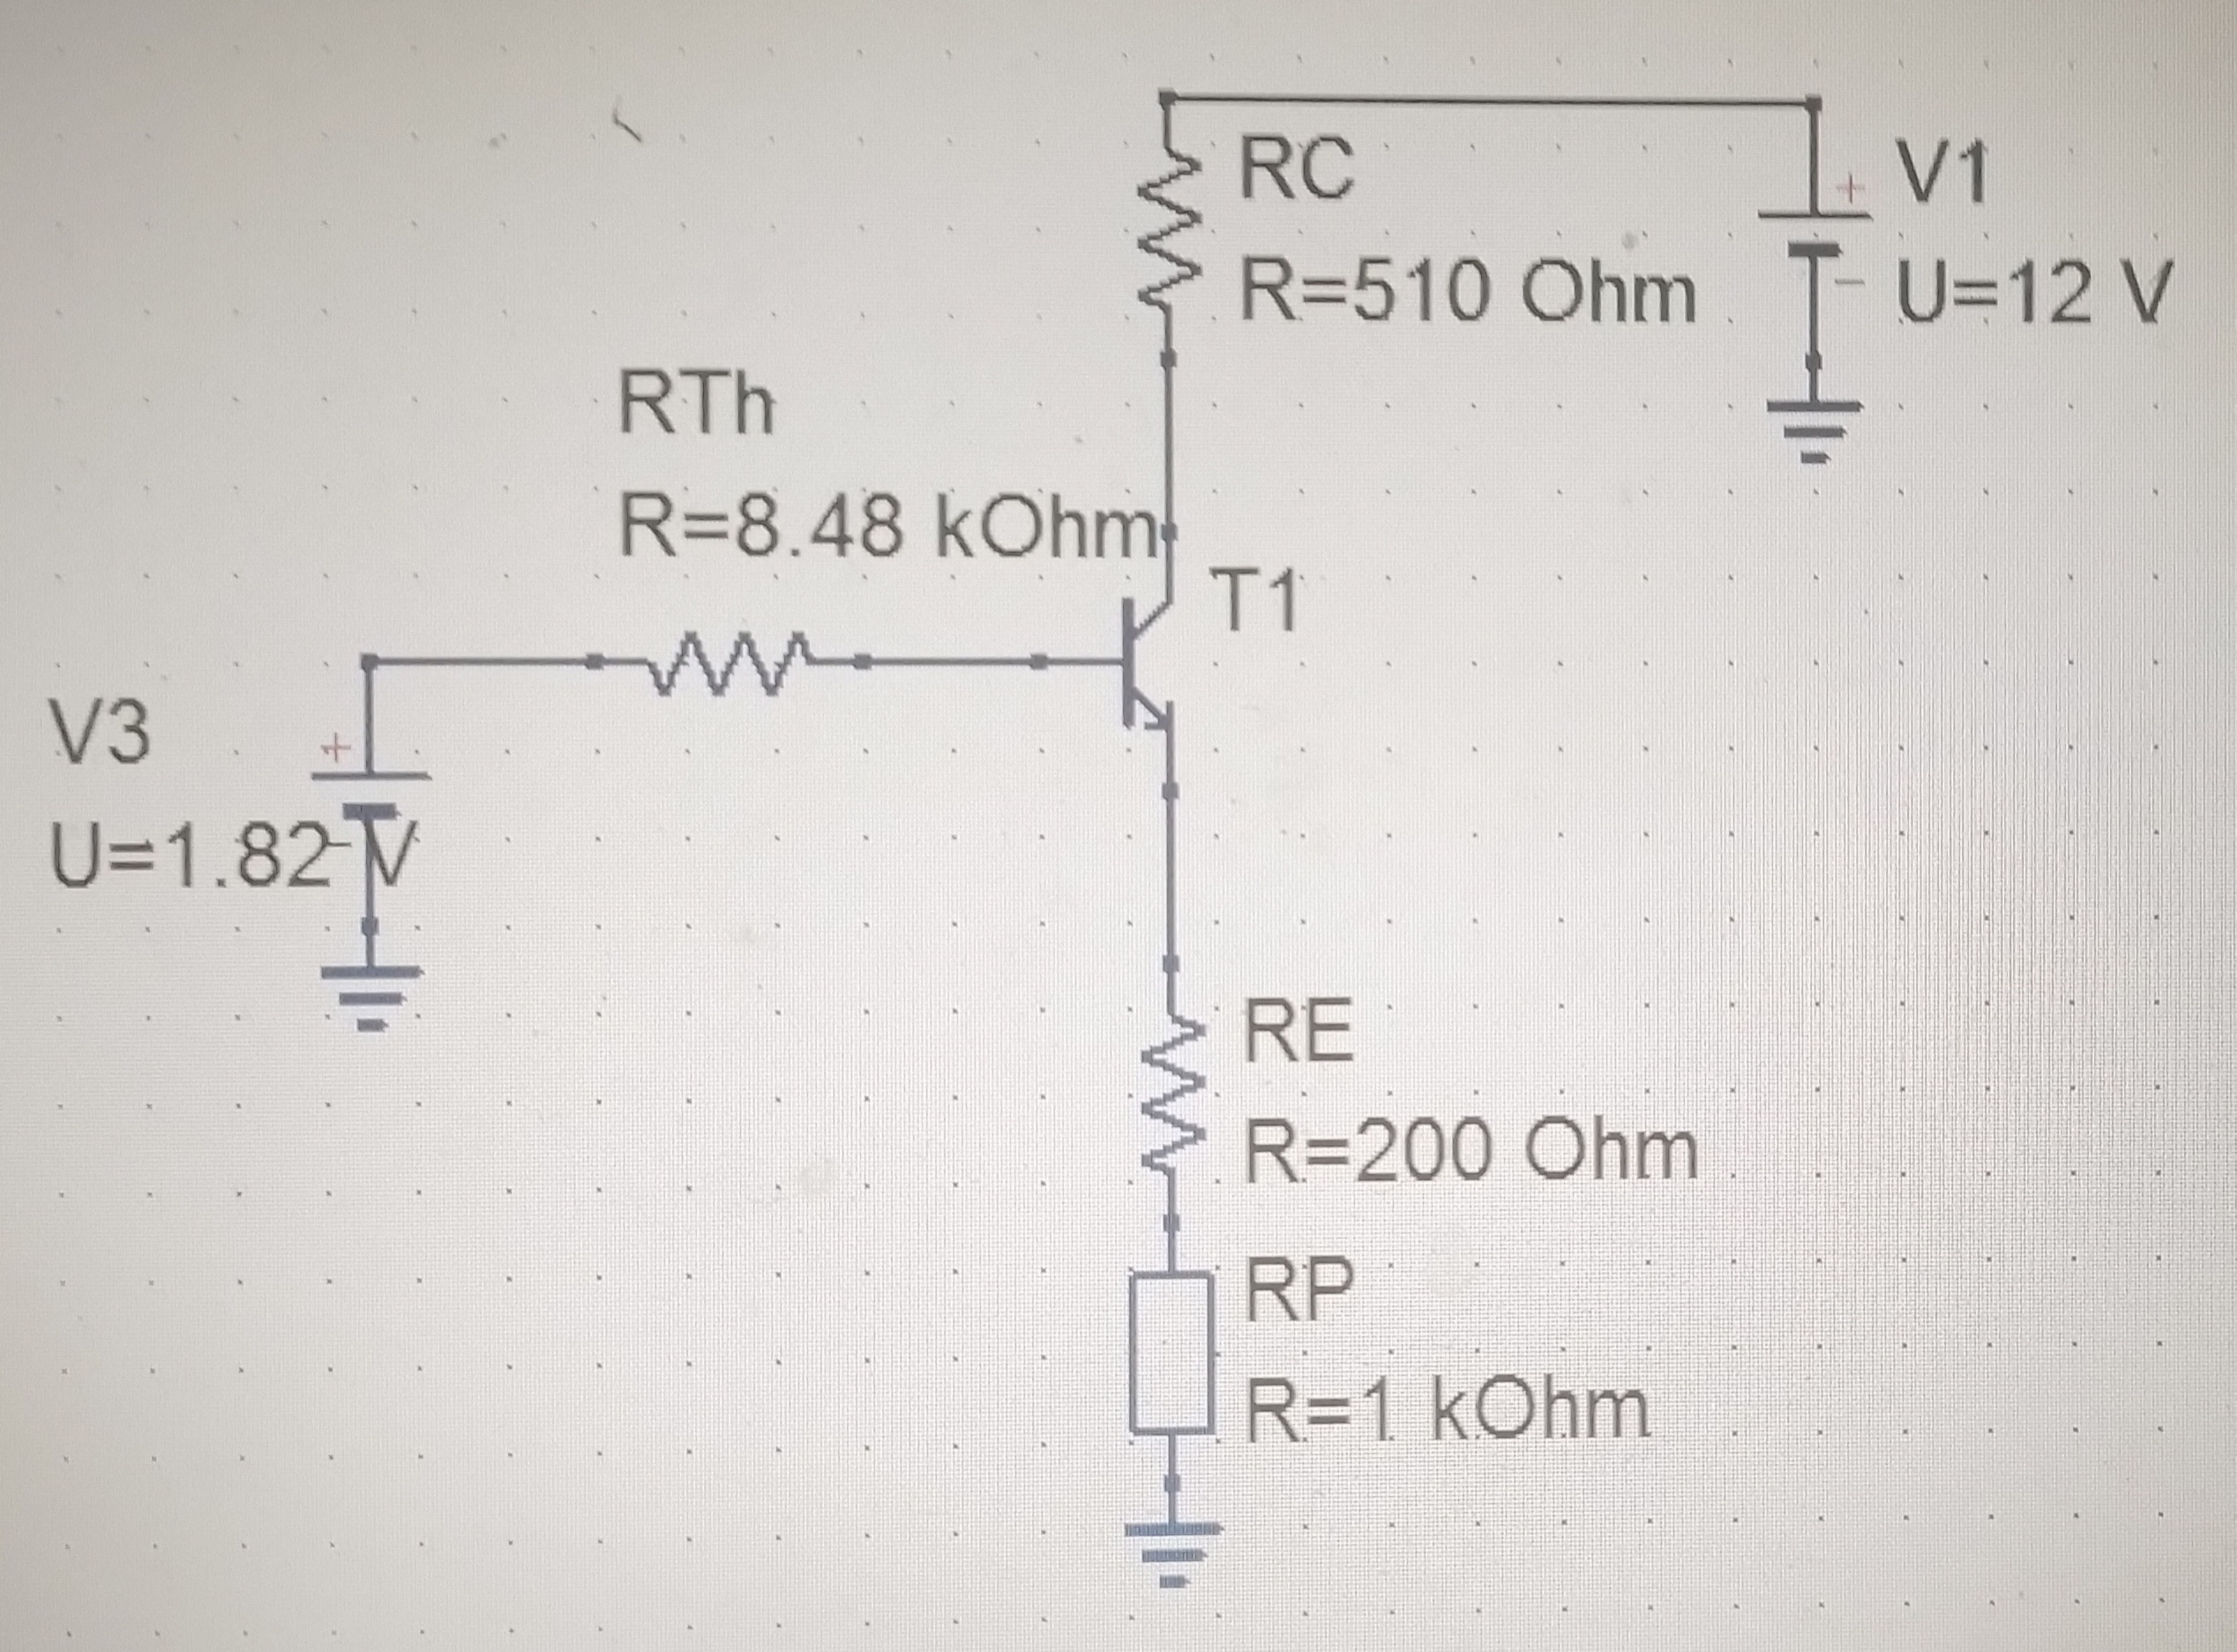
\includegraphics[height=5cm\textwidth]{thevelin6.jpg} \par
        \caption{\label{fig:14} Circuito 6 con equivalente de Thevelin}
    \end{figure}

    aplicando ley de tensiones de Kirchoff

    $$R_{Th}I_B + V_{BE} + (R_E + R_P)I_E = V_{Th}$$

    si $I_E = (\beta + 1)I_B$, entonces

    $$R_{Th}I_B + V_{BE} + (R_E + R_P)(\beta + 1)I_B = V_{Th}$$

    $$I_B = {V_{Th} - V{BE} \over R_{Th} + (R_E + R_P)(\beta + 1)}$$

    Sustituyendo valores

    $$I_B = {1.82V - 0.6V \over 8,48k\Omega + (200\Omega + R_P)(100 + 1)} = {1.22 \over 28680 +101R_P} A$$

    sabiendo que $I_C = \beta I_B$

    $$I_C = 100({1.22 \over 28680 +101R_P})A = {122 \over 28680 +101R_P}A$$

    por otra parte

    $$I_E = (\beta + 1)I_B = (100 + 1)({1.22 \over 28680 +101R_P})A = {123.22 \over 28680 +101R_P}A$$

    aplicando ley de tensiones de Kirchoff a la otra malla

    $$R_{C}I_C + V_{CE} + R_EI_E = V_{CC}$$

    $$V_{CE} = V_{CC} - R_{C}I_C - R_EI_E$$

    sustituyendo

    $$V_{CE} = 12V - 510\Omega ({122 \over 28680 +101R_P}A) - 200\Omega ({123.22 \over 28680 +101R_P}A)$$
    $$V_{CE} = (12 - {86864 \over 28680 +101R_P})V$$

    para caso extremo $R_P = 1k\Omega$

    $$V_{CE} = (12 - {86864 \over 28680 +101(1000)})V = 11.33V$$

    por ley de ohm

    $$V_E = R_EI_E = 200\Omega (0.950mA) = 0.19V$$

    además

    $$V_B = V_{BE} + V_E = 0.7V + 0.19V = 0.89V$$

    $$V_C = V_{CE} + V_E = 11.33V + 0.19V = 11.52V$$

    punto de operacion

    $$Q = (11.33V, 0.940mA)$$

    \newpage

    \section{Materiales}

    \begin{itemize}
        \item Transistor npn PN2222A
        \item Resistencia de carbon de $82k\Omega$  serie del $5\%$ y potencia de ${1/4 W} W$.
        \item Resistencia de carbon de $2k\Omega$  serie del $5\%$ y potencia de ${1/4 W} W$.
        \item Resistencia de carbon de $200\Omega$  serie del $5\%$ y potencia de ${1/4 W} W$.
        \item Resistencia de carbon de $36k\Omega$  serie del $5\%$ y potencia de ${1/4 W} W$.
        \item Resistencia de carbon de $3k\Omega$  serie del $5\%$ y potencia de ${1/4 W} W$.
        \item Resistencia de carbon de $39k\Omega$  serie del $5\%$ y potencia de ${1/4 W} W$.
        \item Resistencia de carbon de $82k\Omega$  serie del $5\%$ y potencia de ${1/4 W} W$.
        \item Resistencia de carbon de $10k\Omega$  serie del $5\%$ y potencia de ${1/4 W} W$.
        \item Resistencia de carbon de $15k\Omega$  serie del $5\%$ y potencia de ${1/4 W} W$.
        \item Resistencia de carbon de $6.8k\Omega$  serie del $5\%$ y potencia de ${1/4 W} W$.
        \item Resistencia de carbon de $300\Omega$  serie del $5\%$ y potencia de ${1/4 W} W$.
        \item Resistencia de carbon de $130\Omega$  serie del $5\%$ y potencia de ${1/4 W} W$.
        \item Resistencia de carbon de $300\Omega$  serie del $5\%$ y potencia de ${1/4 W} W$.
        \item Resistencia de carbon de $300\Omega$  serie del $5\%$ y potencia de ${1/4 W} W$.
        \item Resistencia de carbon de $300\Omega$  serie del $5\%$ y potencia de ${1/4 W} W$.
    \end{itemize}

\end{document}